\documentclass[12pt]{article}


\usepackage{amssymb}
\usepackage{amsmath}
\usepackage{fullpage}
\usepackage{epsfig}
\usepackage{epstopdf}
\everymath{\displaystyle}
\usepackage{enumerate}



\begin{document}

\begin{center}
\underline{\LARGE{Vectors \& Vector Arithmetic}}
\end{center}

\noindent SUGGESTED REFERENCE MATERIAL:

\bigskip

\noindent As you work through the problems listed below, you should reference Chapter 11.2 of the recommended textbook (or the equivalent chapter in your alternative textbook/online resource) and your lecture notes.

\bigskip

\noindent EXPECTED SKILLS:

\begin{itemize}

\item Be able to perform arithmetic operations on vectors and understand the geometric consequences of the operations. 

\item Know how to compute the magnitude of a vector and normalize a vector. 

\item Be able to use vectors in the context of geometry and force problems.

\end{itemize}

\noindent PRACTICE PROBLEMS:

\medskip

\begin{enumerate}

\item Find the components of vector $\overrightarrow{v}$ and sketch an equivalent vector with its initial point at the origin.

\begin{center}
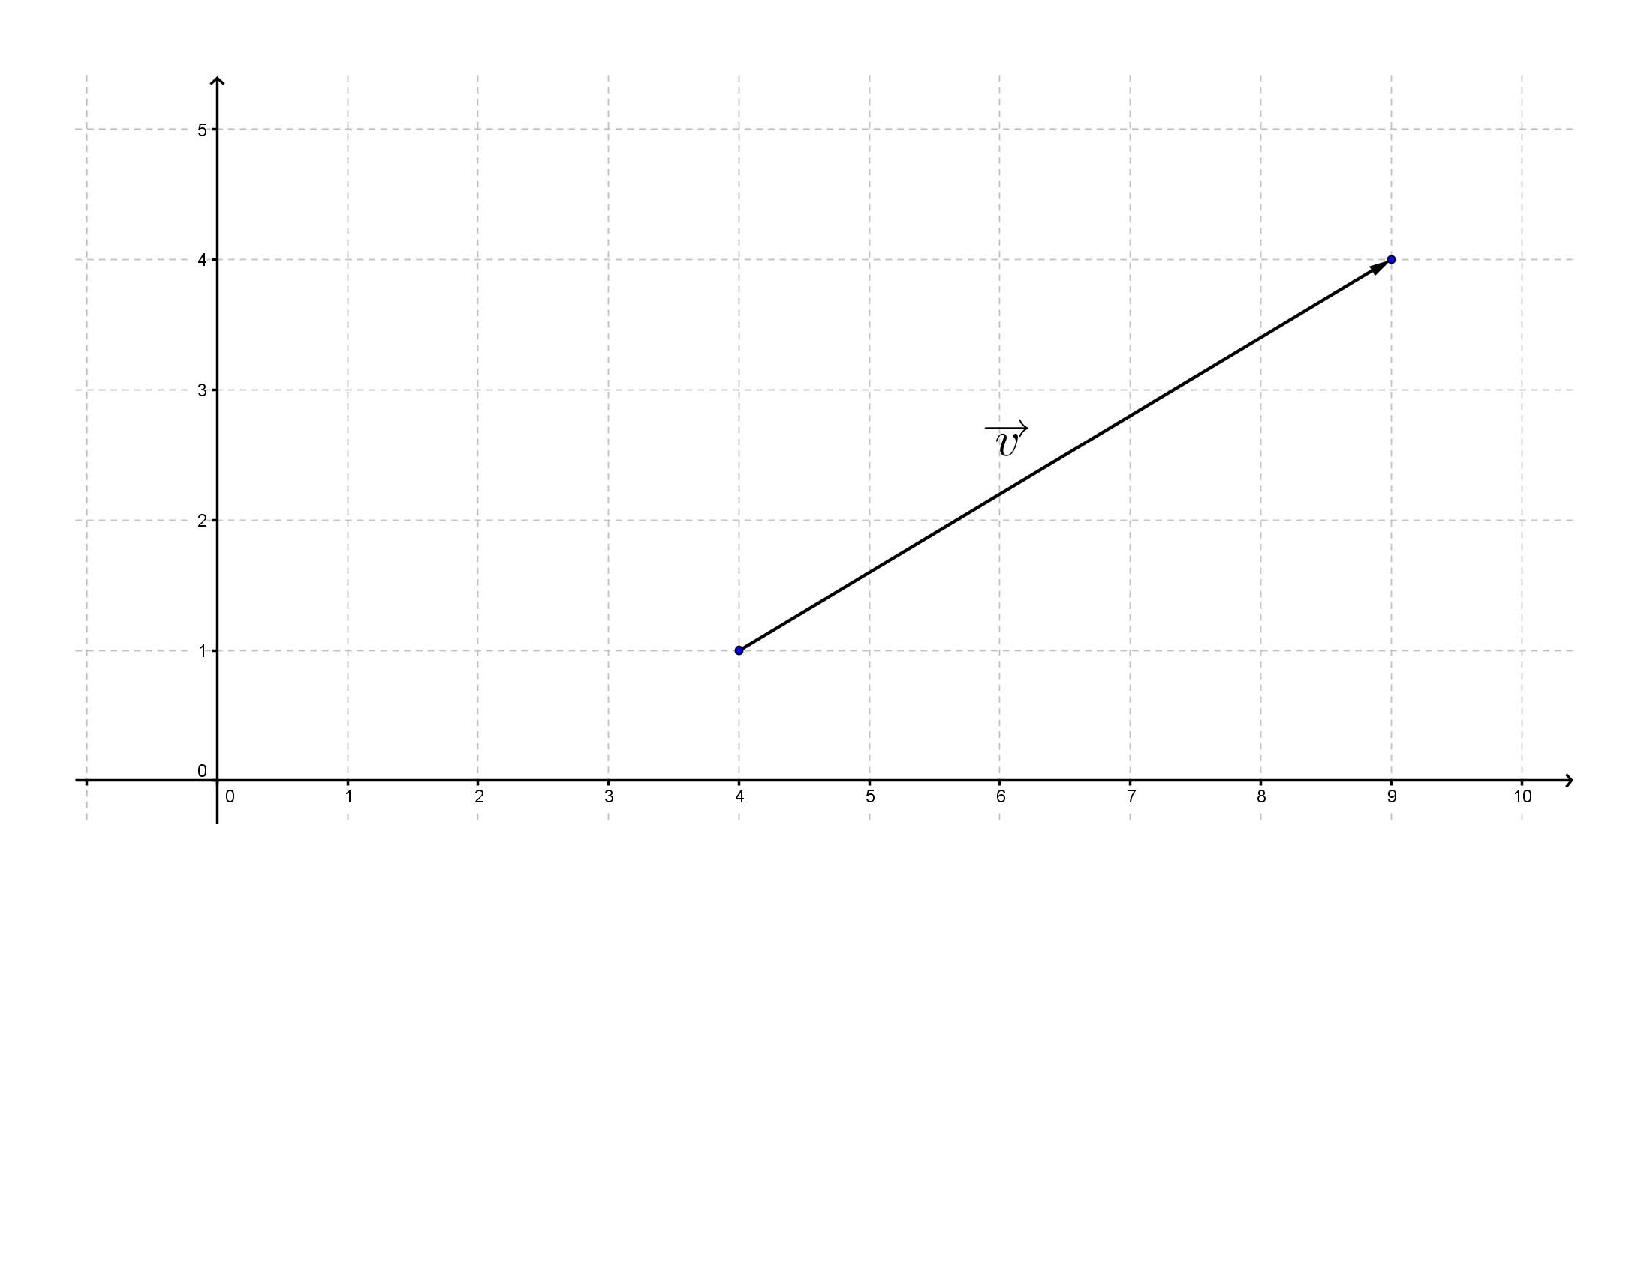
\includegraphics[scale=0.4]{vector1.pdf}
\end{center}

\includegraphics[scale=0.5]{start.pdf}
{{{0.75\linewidth}{\begin{center}$\overrightarrow{v}=\langle 5,3 \rangle$\\
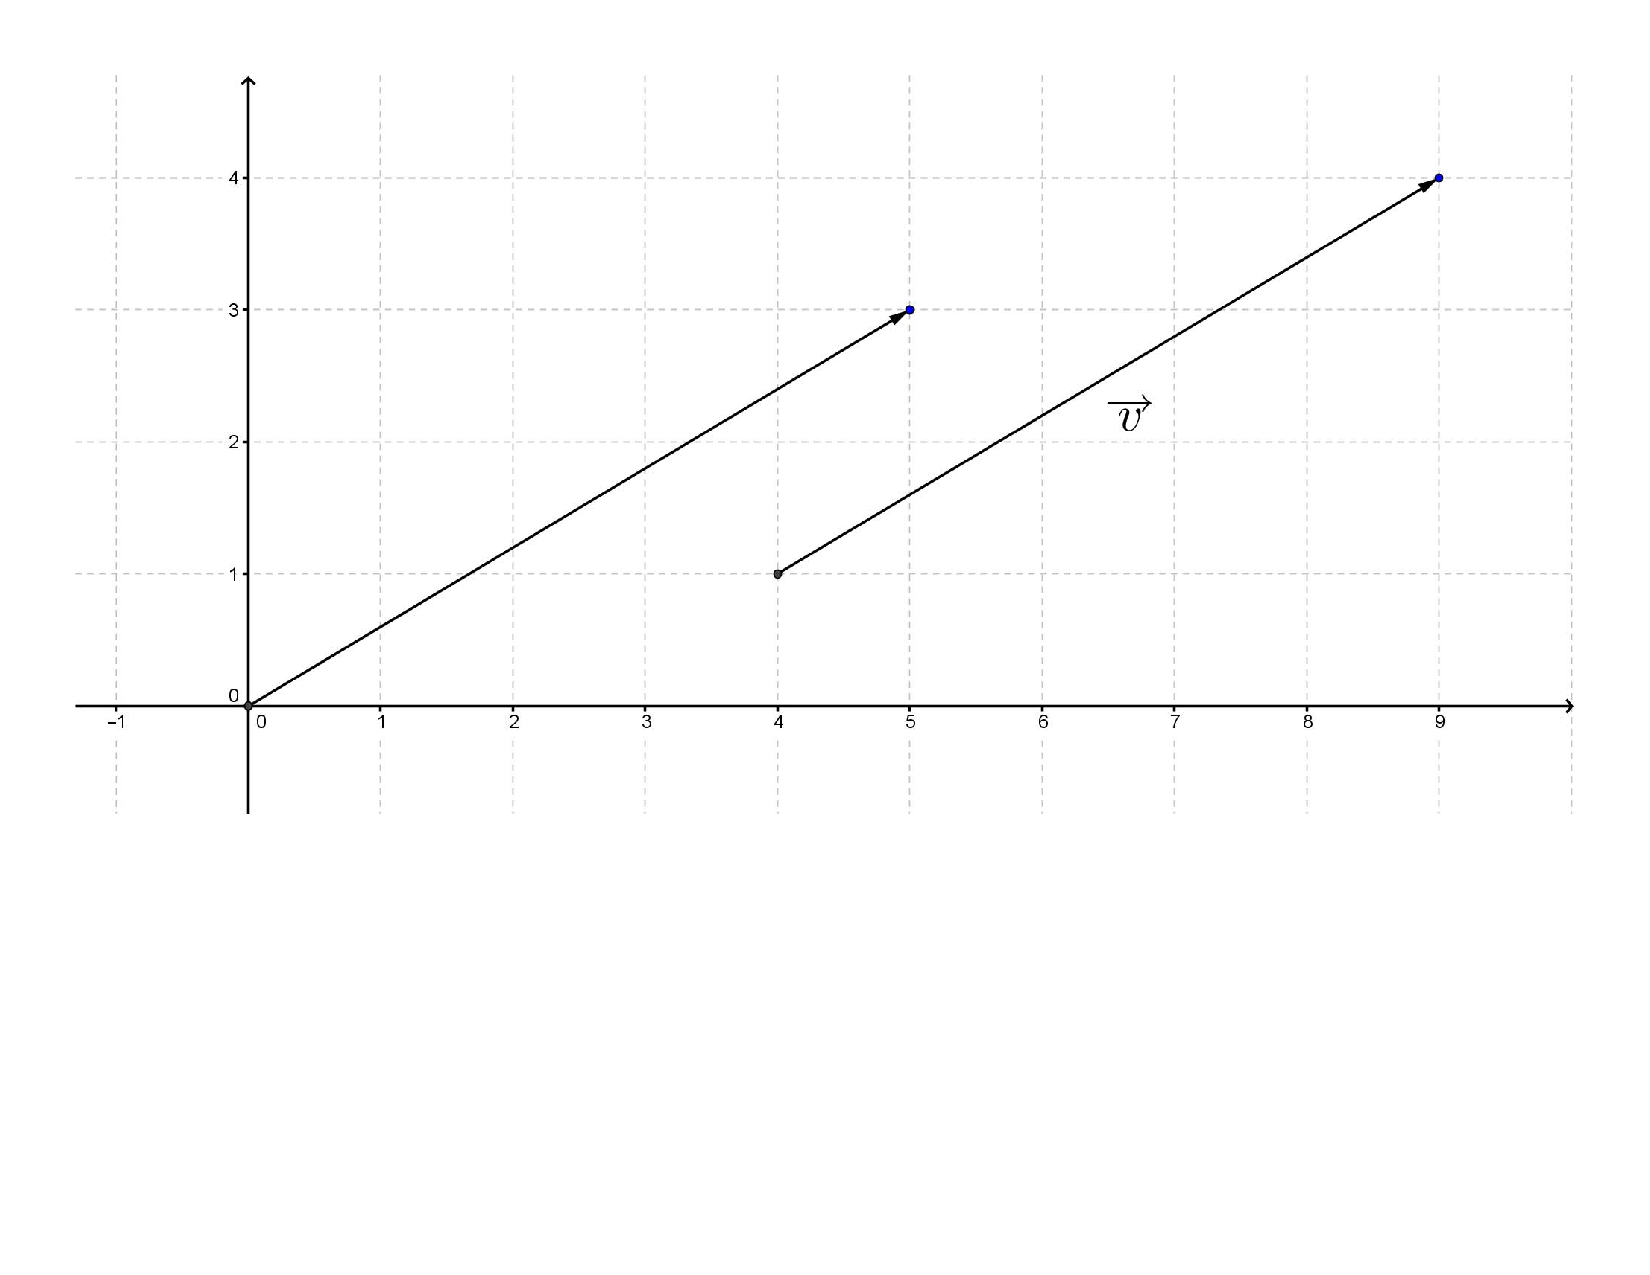
\includegraphics[scale=0.3]{vector1ans.pdf}\end{center}}}}
\includegraphics[scale=0.5]{end.pdf}


\item Sketch the vector $\overrightarrow{u}+\overrightarrow{v}+\overrightarrow{w}$ and express it in component form.

\begin{center}
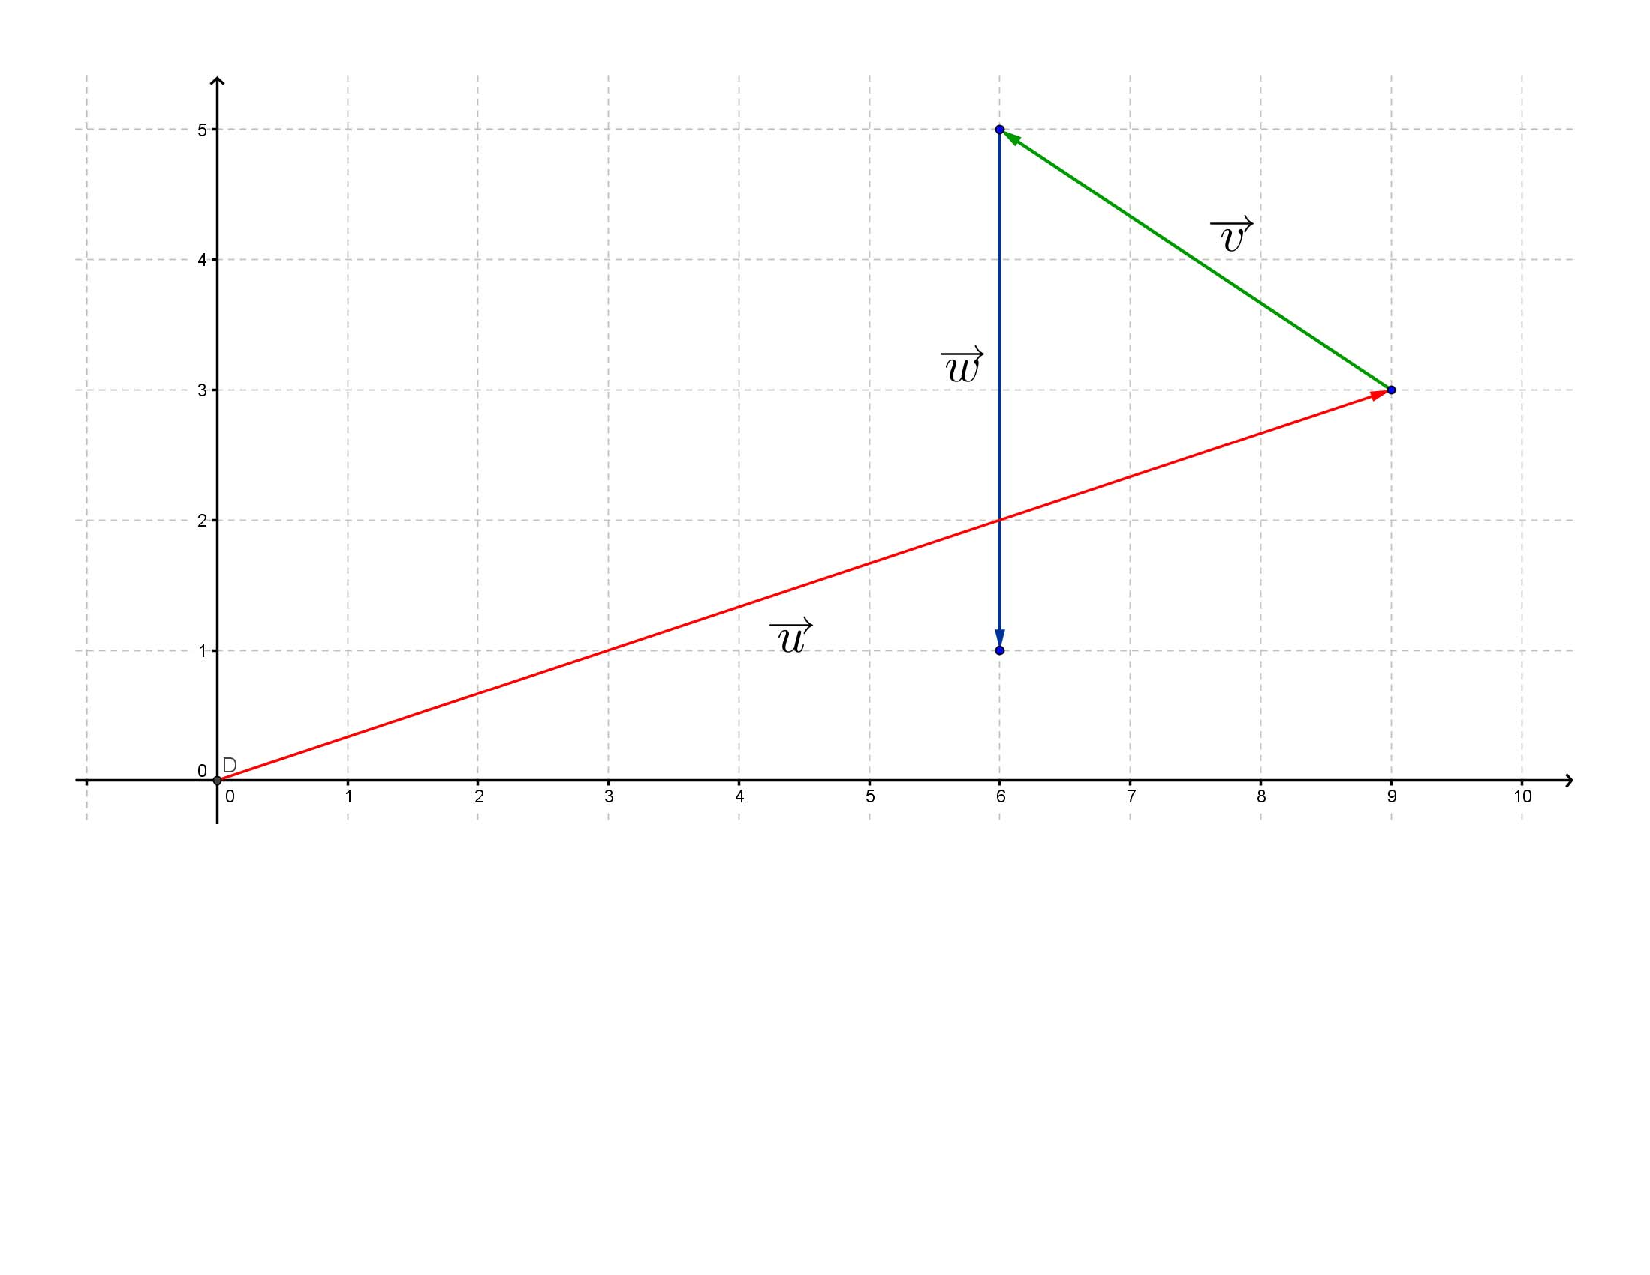
\includegraphics[scale=0.4]{vector2.pdf}
\end{center}

\includegraphics[scale=0.5]{start.pdf}
{{{0.75\linewidth}{\begin{center}$\overrightarrow{u}+\overrightarrow{v}+\overrightarrow{w}=\langle 6,1 \rangle$\\
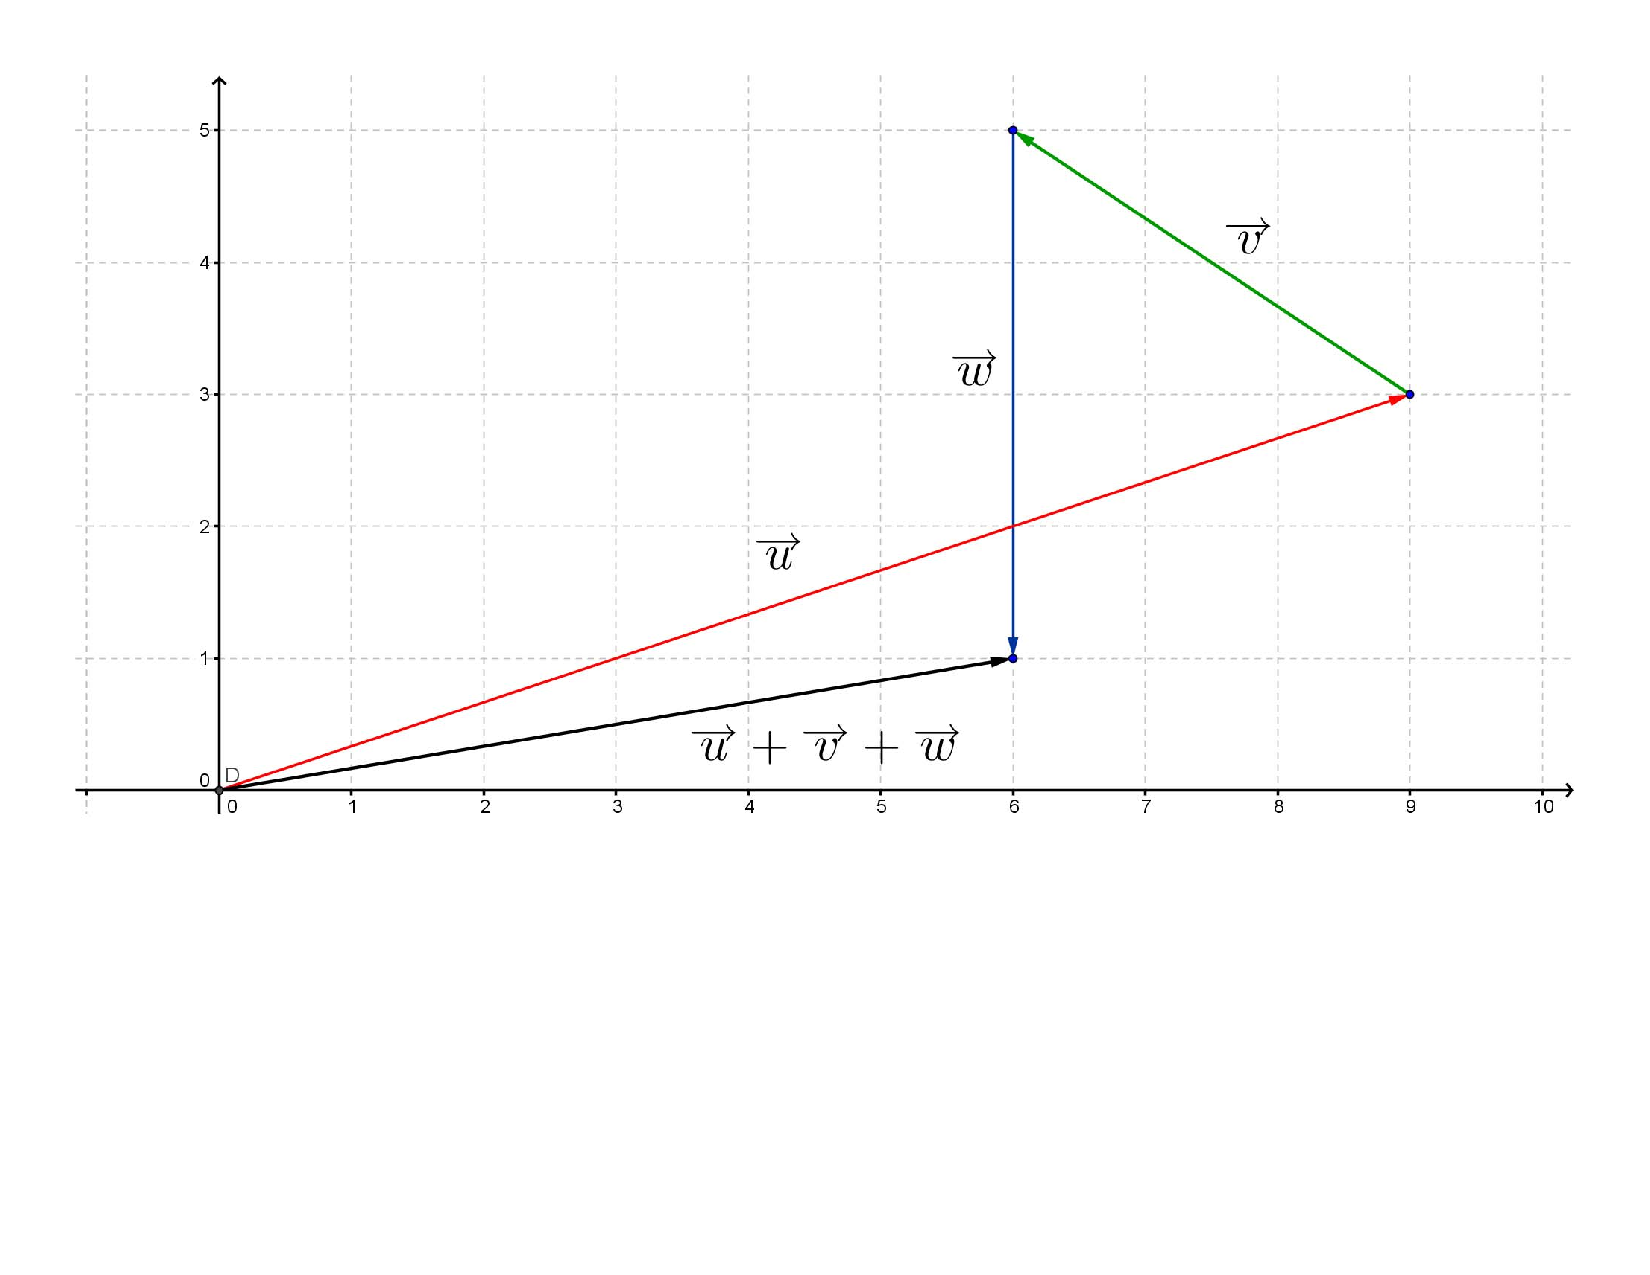
\includegraphics[scale=0.3]{vector2ans.pdf}\end{center}}}}
\includegraphics[scale=0.5]{end.pdf}


\item The figure below is a parallelogram.  Express $\overrightarrow{w}$ in terms of $\overrightarrow{u}$ and $\overrightarrow{v}$.

\begin{center}
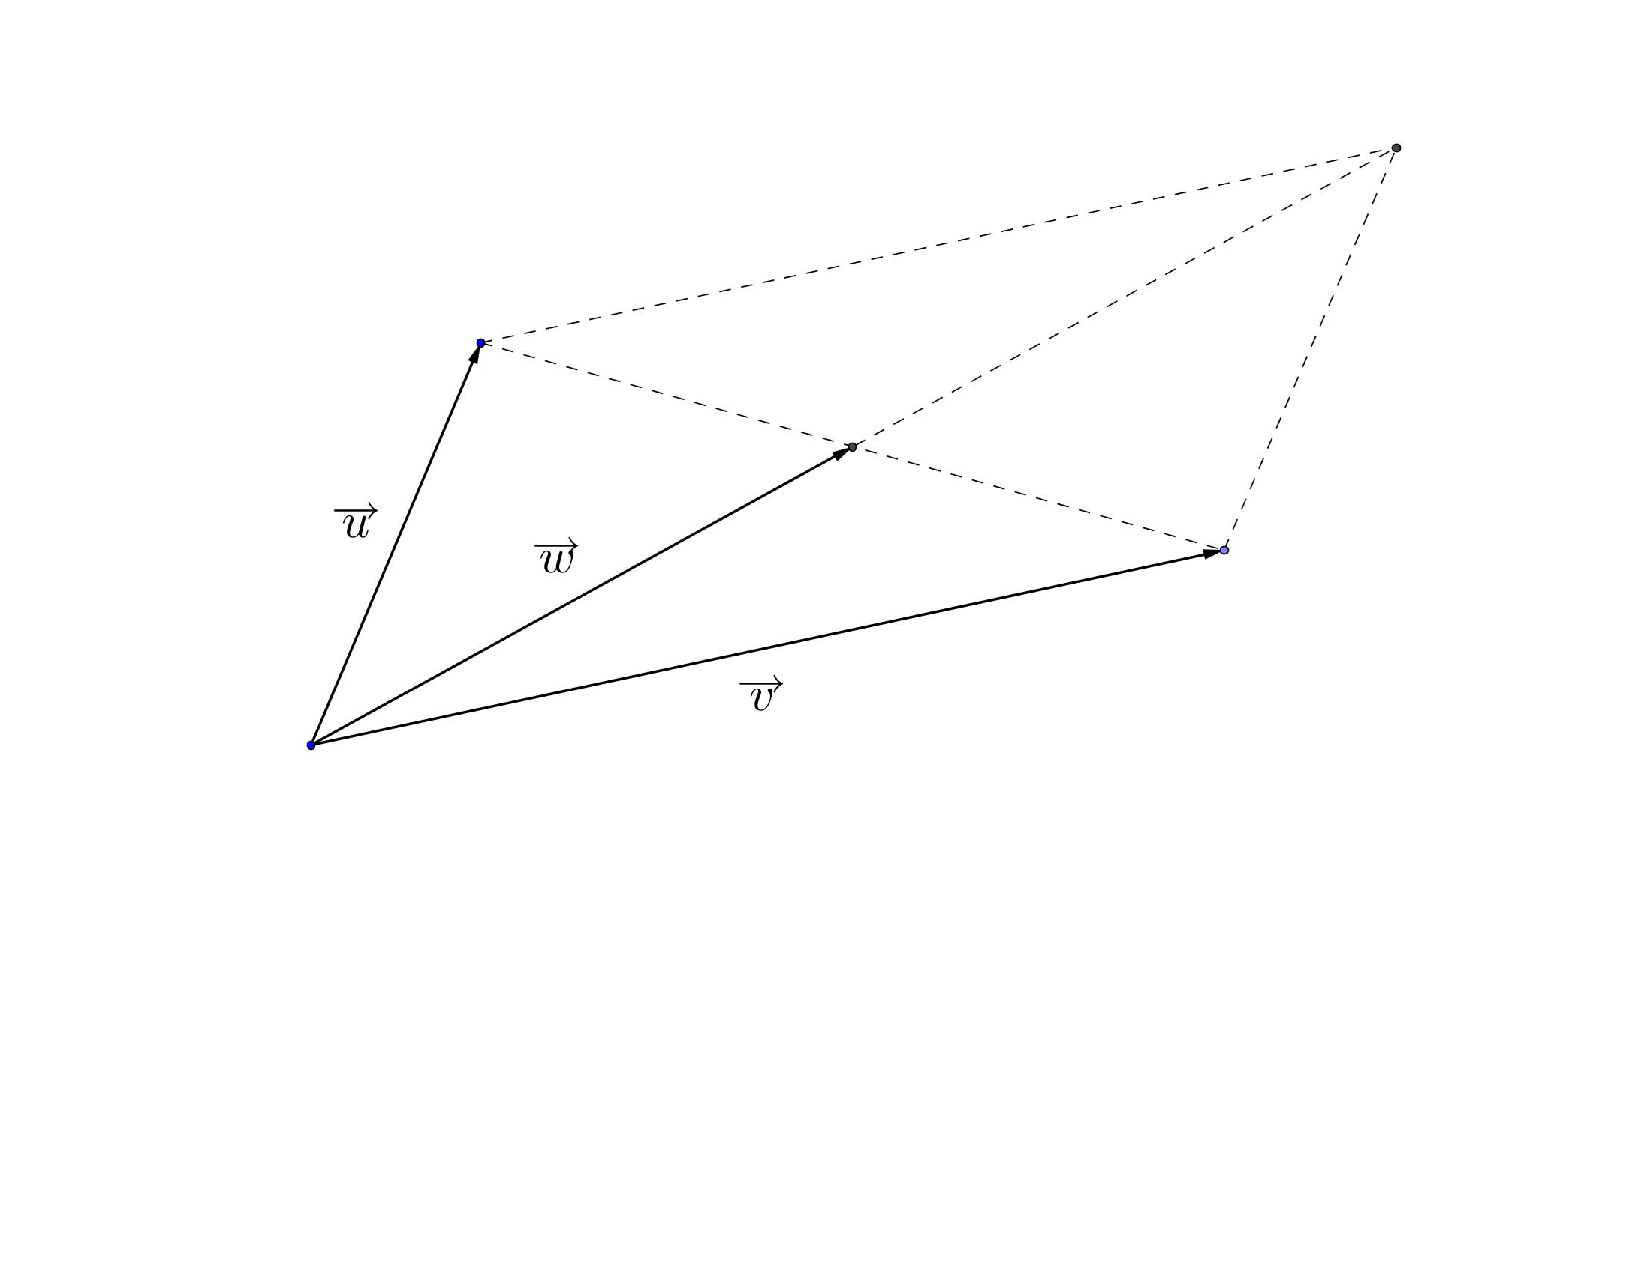
\includegraphics[scale=0.4]{vector3.pdf}
\end{center}

\includegraphics[scale=0.5]{start.pdf}
{{$\overrightarrow{w}=\frac{1}{2}\left(\overrightarrow{u}+\overrightarrow{v}\right)$}}
\includegraphics[scale=0.5]{end.pdf}


\item Consider the points $P_1(2,3)$ and $P_2=(5,-1)$. Find the components of the vector $\overrightarrow{P_1P_2}$.  Sketch $P_1$, $P_2$, $\overrightarrow{P_1P_2}$, and an equivalent vector with its initial point at the origin.

\includegraphics[scale=0.5]{start.pdf}
{{{0.75\linewidth}{\begin{center}$\overrightarrow{P_1P_2}=\langle 3,-4 \rangle$\\
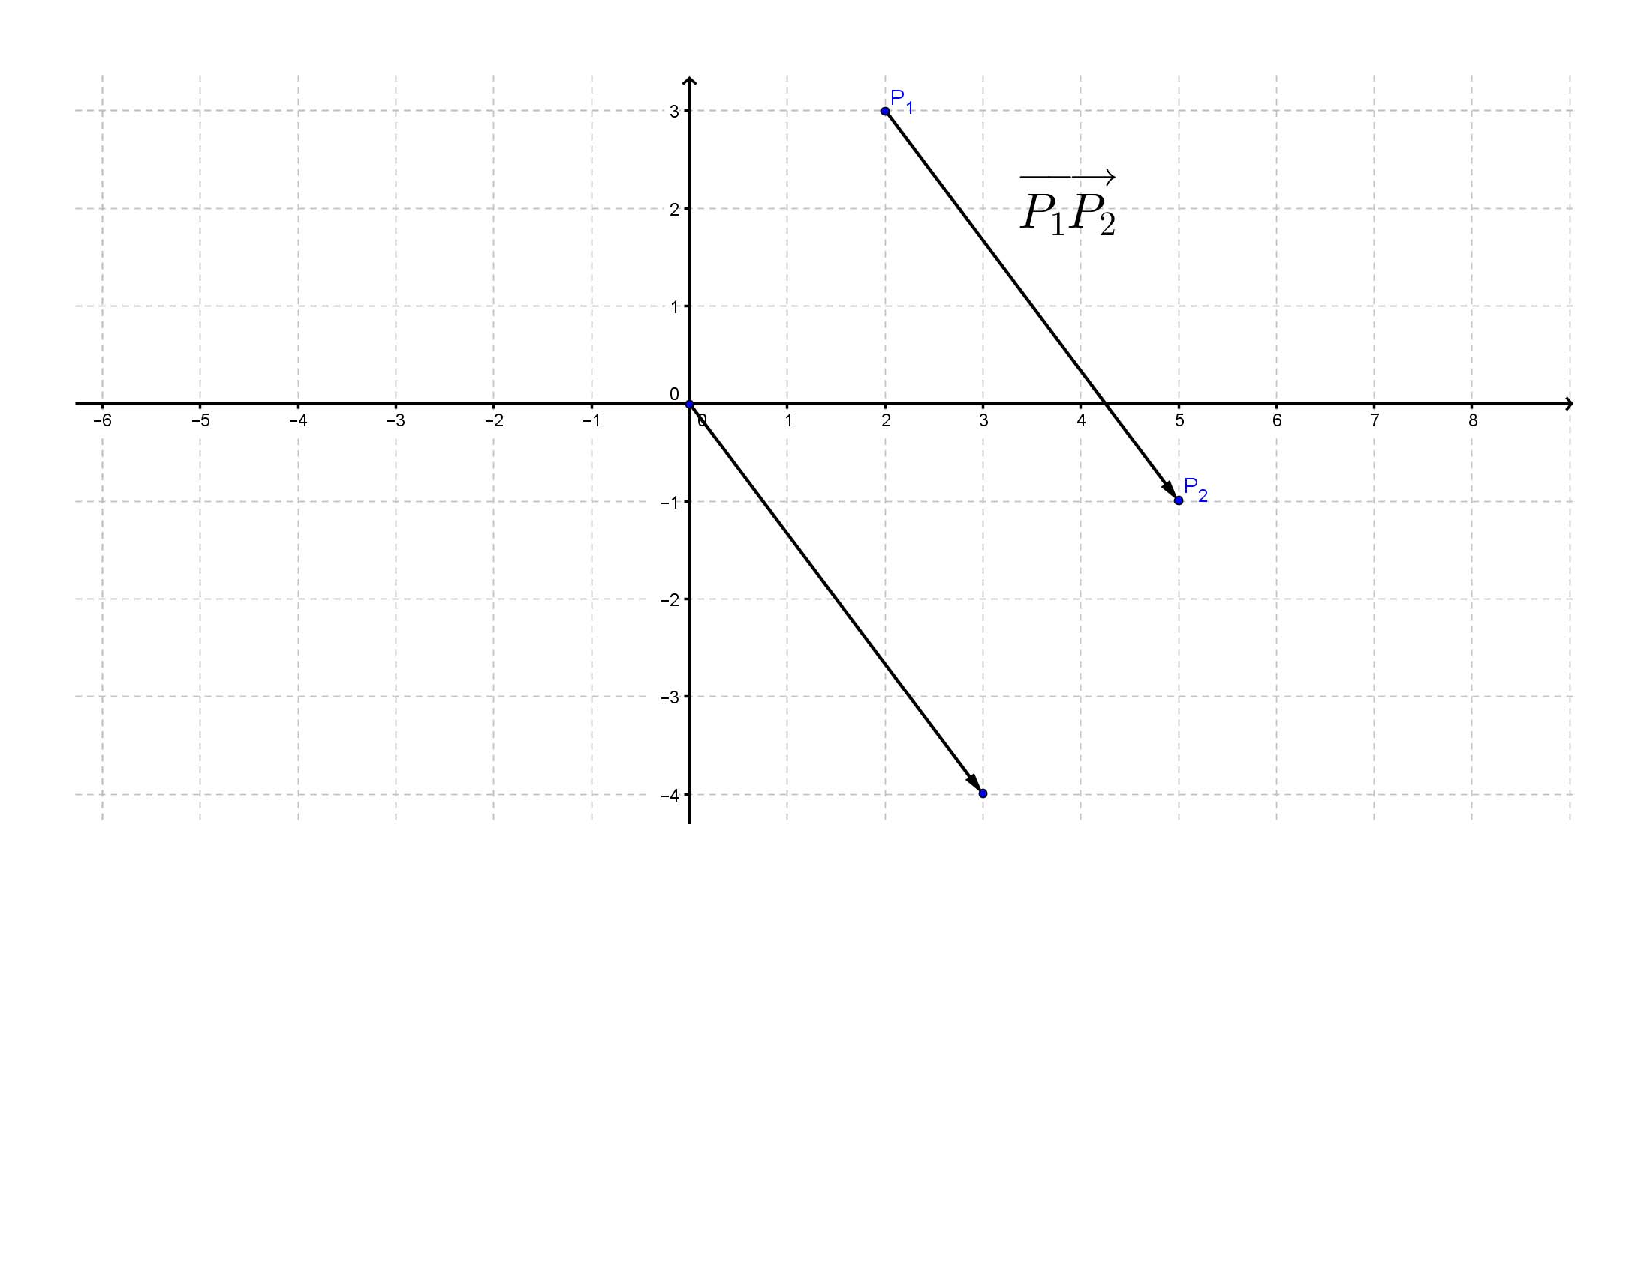
\includegraphics[scale=0.3]{vector4.pdf}\end{center} }}}
\includegraphics[scale=0.5]{end.pdf}


\item Consider the points $P_1(1,2,3)$ and $P_2(5,4,6)$.  Find the components of the vector $\overrightarrow{P_1P_2}$.

\includegraphics[scale=0.5]{start.pdf}
{{$\overrightarrow{P_1P_2}=\langle 4,2,3 \rangle$}}
\includegraphics[scale=0.5]{end.pdf}


\item Let ${\bf u}= 3{\bf i}+2{\bf j}-{\bf k}$, ${\bf v}=-2{\bf i}+4{\bf j}+3{\bf k}$, and ${\bf w}=7{\bf i}+4{\bf j}+{\bf k}$.  Compute each of the following:

\begin{enumerate}

\item $2{\bf u}-3{\bf w}$

\includegraphics[scale=0.5]{start.pdf}
{{$-15{\bf i}-8{\bf j}-5{\bf k}$}}
\includegraphics[scale=0.5]{end.pdf}


\item $\| {\bf u}+{\bf v}\|$

\includegraphics[scale=0.5]{start.pdf}
{{$\sqrt{41}$}}
\includegraphics[scale=0.5]{end.pdf}


\item $\| {\bf u}\|+\|{\bf v}\|$

\includegraphics[scale=0.5]{start.pdf}
{{$\sqrt{14}+\sqrt{29}$}}
\includegraphics[scale=0.5]{end.pdf}


\item $\|2{\bf u}\|$

\includegraphics[scale=0.5]{start.pdf}
{{$2\sqrt{14}$}}
\includegraphics[scale=0.5]{end.pdf}


\item $\left\|\frac{1}{\|{\bf v}\|}{\bf v}\right\|$

\includegraphics[scale=0.5]{start.pdf}
{{1}}
\includegraphics[scale=0.5]{end.pdf}


\end{enumerate}

\item For each of the following, find a vector which satisfies the given conditions.

\begin{enumerate}

\item A unit vector which is in the opposite direction of ${\bf v}=3{\bf i}+4{\bf j}$

\includegraphics[scale=0.5]{start.pdf}
{{$-\frac{3}{5}{\bf i}-\frac{4}{5}{\bf j}$}}
\includegraphics[scale=0.5]{end.pdf}


\item A unit vector which is in the same direction as the vector from $P_1(1,0,5)$ to $P_2(3,-1,2)$

\includegraphics[scale=0.5]{start.pdf}
{{$\left \langle \frac{2}{\sqrt{14}},-\frac{1}{\sqrt{14}},-\frac{3}{\sqrt{14}} \right \rangle$}}
\includegraphics[scale=0.5]{end.pdf}


\item A vector which is in the opposite direction of $\overrightarrow{v}=\langle1,2,3\rangle$ and whose maginitude is half that of $\overrightarrow{v}$.

\includegraphics[scale=0.5]{start.pdf}
{{$\left \langle -\frac{1}{2},-1,-\frac{3}{2}\right\rangle$}}
\includegraphics[scale=0.5]{end.pdf}


\item A vector which is in the same direction of ${\bf w}={\bf i}-2{\bf j}+3{\bf k}$ and which has a length of $\sqrt{5}$

\includegraphics[scale=0.5]{start.pdf}
{{$\frac{\sqrt{5}}{\sqrt{14}}{\bf i}-\frac{2\sqrt{5}}{\sqrt{14}}{\bf j}+\frac{3\sqrt{5}}{\sqrt{14}}{\bf k}$}}
\includegraphics[scale=0.5]{end.pdf}


\item A vector in 2-space which makes an angle of $\theta=\frac{\pi}{6}$ with the positive $x$-axis and which has a magnitude of 4.

\includegraphics[scale=0.5]{start.pdf}
{{$\left \langle 2\sqrt{3}, 2 \right \rangle$}}
\includegraphics[scale=0.5]{end.pdf}


\item A vector in 2-space which makes an angle of $\theta=210^{\circ}$ with the positive $x$-axis and which has a length of 2.

\includegraphics[scale=0.5]{start.pdf}
{{$\left \langle -\sqrt{3},-1 \right \rangle$}}
\includegraphics[scale=0.5]{end.pdf}


\end{enumerate}

\item Find the value(s) of $a$ so that the vectors $\overrightarrow{v}=\langle a^2,6 \rangle$ and $\overrightarrow{w}=\langle 4a, 2 \rangle$ are parallel.

\includegraphics[scale=0.5]{start.pdf}
{{$a=0$ or $a=12$}}
\includegraphics[scale=0.5]{end.pdf}


\item Vectors $\overrightarrow{v}$ and $\overrightarrow{w}$, shown below, are unit vectors.  Find the components of $\overrightarrow{v}+\overrightarrow{w}$.

\begin{center}
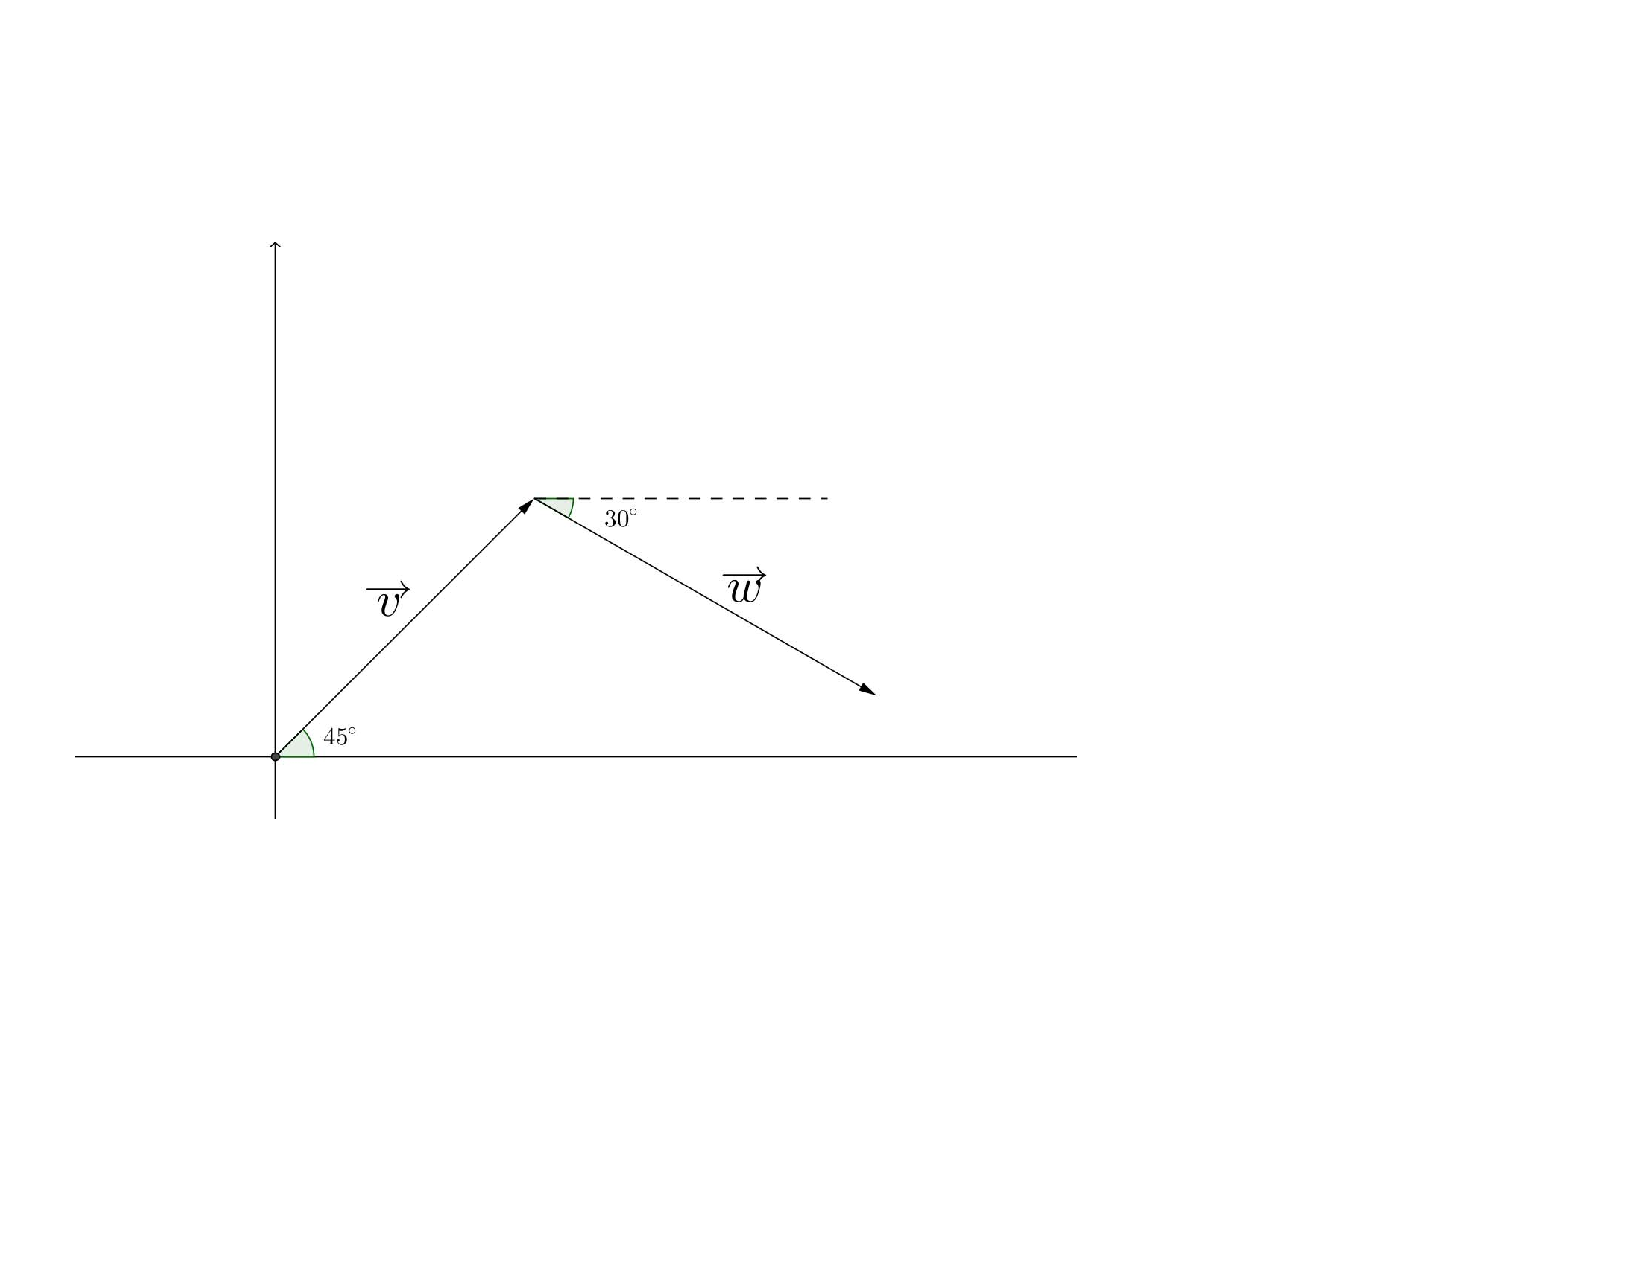
\includegraphics[scale=0.5]{vector5.pdf}
\end{center}

\includegraphics[scale=0.5]{start.pdf}
{{$\left \langle \frac{\sqrt{2}+\sqrt{3}}{2},\frac{\sqrt{2}-1}{2}\right \rangle$}}
\includegraphics[scale=0.5]{end.pdf}


\item For each of the following, find the magnitude of the resultant force and the angle that it makes with the positive $x$-axis.

\begin{tabular}{ll}
(a) & \\
 & 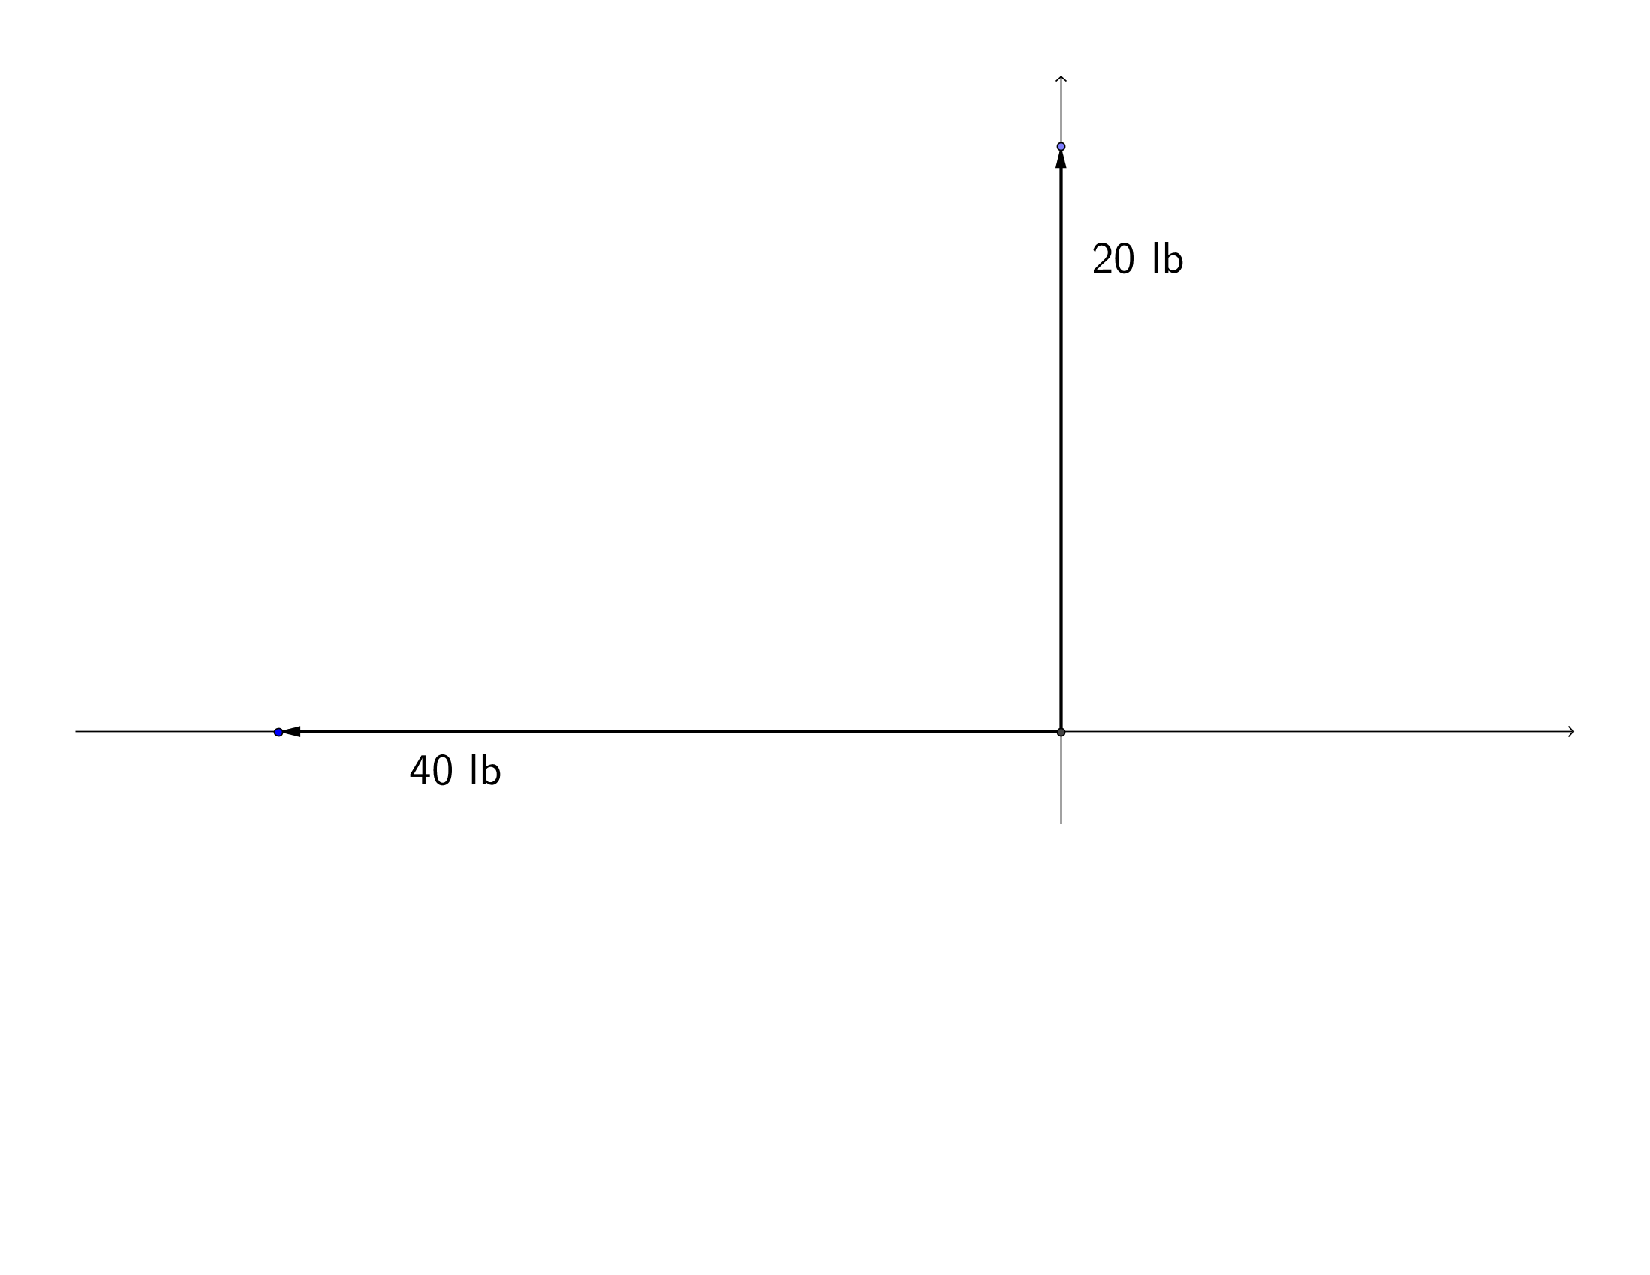
\includegraphics[scale=0.4]{vector7.pdf}\\
(b) & \\
 & 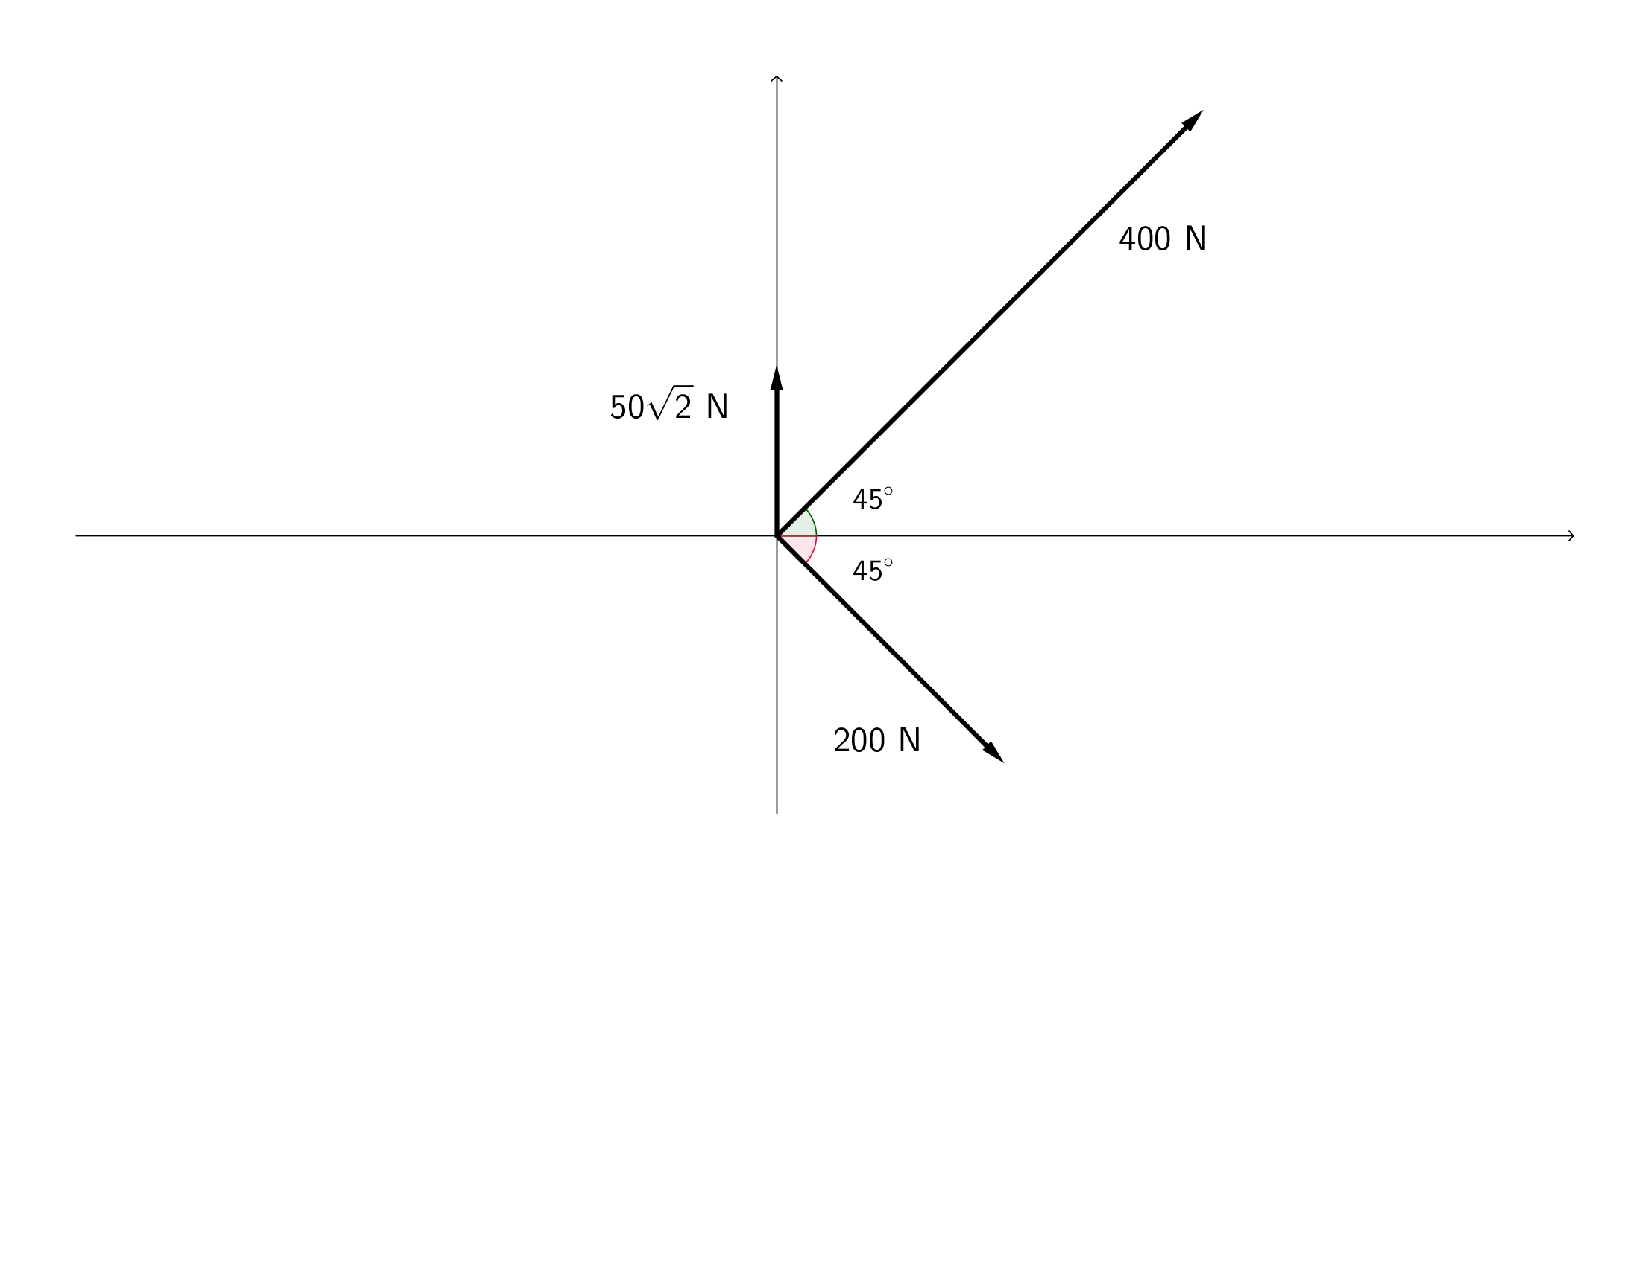
\includegraphics[scale=0.4]{vector8.pdf}\\
\end{tabular}

\includegraphics[scale=0.5]{start.pdf}
{{{1\linewidth}{(a) The magnitude is $20\sqrt{5}$ lb at an angle of $\pi-\tan^{-1}\left(\frac{1}{2}\right)$ radians counterclockwise with the positive $x$ axis.\\
\\
(b) The magnitude is $150\sqrt{10}$ N at an angle of $\tan^{-1}\left(\frac{1}{2}\right)$ radians counterclockwise with the positive $x$ axis.}}}
\includegraphics[scale=0.5]{end.pdf}


\newpage

\item A weight of 200 Newtons (N) is being supported by two wires, as shown below.  Find the tension in each wire.
\begin{center}
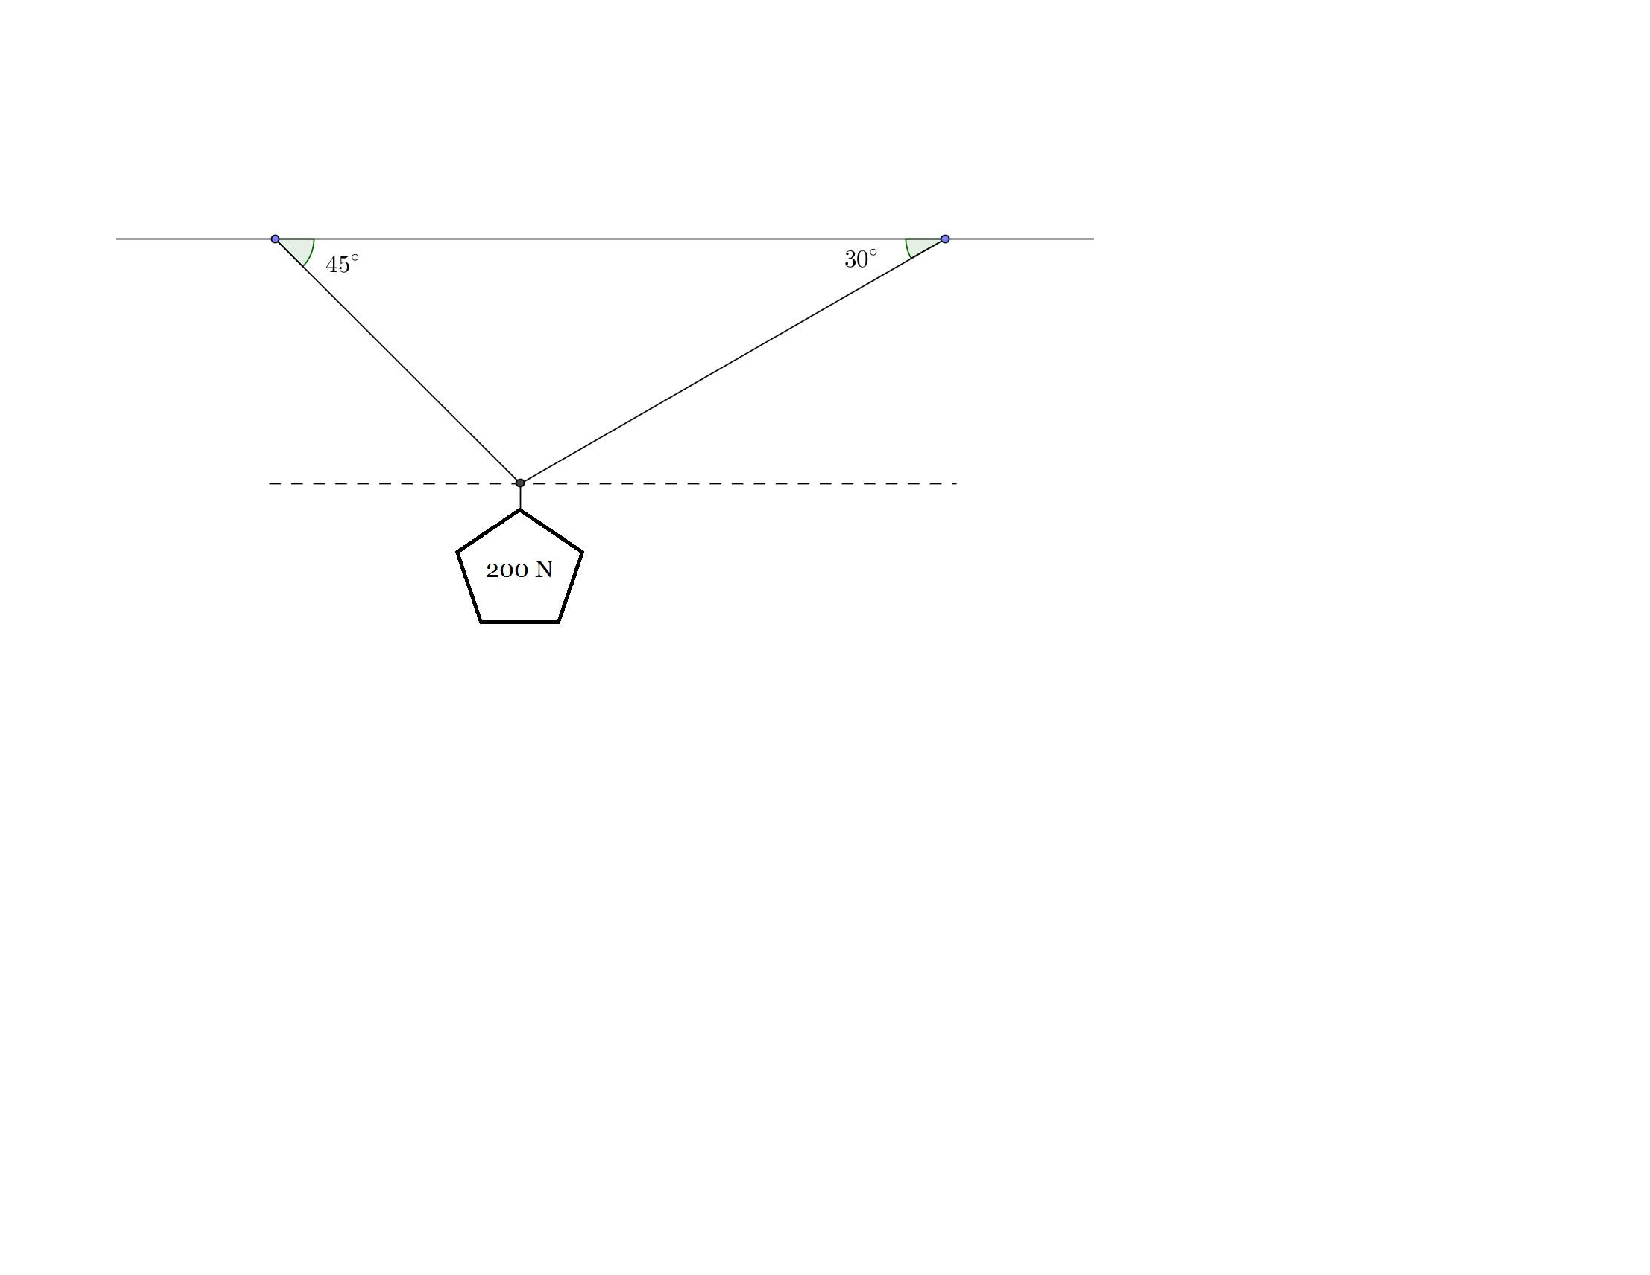
\includegraphics[scale=0.6]{vector6.pdf}
\end{center}

\includegraphics[scale=0.5]{start.pdf}
{{{1\linewidth}{Let $F_1$ be the wire which  makes an angle of $45^{\circ}$ clockwise with the ceiling and $F_2$ be the wire which  makes an angle of $30^{\circ}$ counterclockwise with the ceiling.  Then $\|F_2\|=\frac{400}{1+\sqrt{3}}$ N and $\|F_1\|=\frac{\sqrt{3}}{\sqrt{2}}\cdot\frac{400}{1+\sqrt{3}}$ N.}}}
\includegraphics[scale=0.5]{end.pdf}


\end{enumerate}

\end{document}